The electronics that modern computers rely on contain components that operate based on quantum mechanics; however, their computational processes are still governed by classical laws. 
For this reason, they are referred to as "classical computers."\\

Quantum computing emerged from Richard Feynman’s idea that simulating quantum systems efficiently requires quantum mechanical resources \cite{Feynman1982}. 
Classical computers struggle to model complex quantum interactions due to the exponential growth of computational requirements with system size, making exact simulations infeasible beyond small systems \cite{Brown2010}. 
Quantum computers, taking advantage of quantum mechanics phenomena like superposition and entanglement, offer a natural framework for such simulations and have been demonstrated to provide exponential speedups for certain quantum systems \cite{Georgescu_2014}.

Beyond quantum simulation, curren theoretical advancements suggest that quantum algorithms can outperform classical counterparts in solving specific problems \cite{Montanaro2016}.

\section{Introduction}
The physical realization of quantum computing necessitates the development of a system capable of functioning as quantum bits (qubits).\\
Similar to classical logic, where the bits 0 and 1 are associated with two physical levels, typically represented by high and low voltage states, a qubit can, to a first approximation, be considered as a two-level physical system.

Mathematically, this system is described within a two-dimensional complex Hilbert space, where the basis states $\ket{0}$ and $\ket{1}$ correspond to two orthonormal vectors.
Any general state of the qubit can be expressed as a superporition of these basis states:
\begin{equation}\label{eq:qubit}
    \ket{\psi} = \alpha\ket{0} + \beta\ket{1} \rightarrow \begin{pmatrix} 
        \alpha \\ 
        \beta 
        \end{pmatrix},
\end{equation}
where $\alpha,\beta\in \mathbb{C}$. If the normalization condition $|\alpha|^2 +|\beta|^2 =1$ holds, the state $\ket{\psi}$ represents a qubit.
The basis $\{\ket{0},\ket{1}\}$ is called computational basis and the information is stored in the complex numbers $\alpha$ and $\beta$.

\paragraph{}
A possible geometric representation of qubit states is given by the Bloch sphere, which offers a visualization of two level quantum systems as vectors on a unit sphere.  
A qubit state is depicted as a vector originating from the center of the sphere, with the computational basis states $\ket{0}$ and $\ket{1}$ positioned at the north and south poles, respectively.
The axis connecting these states defines the $z$-axis. The transverse $x$- and $y$- axes correspond to the equal superposition states $\ket{\pm} = \frac{1}{\sqrt{2}}(\ket{0}\pm\ket{1})$ and $\ket{\pm i} = \frac{1}{\sqrt{2}}(\ket{0}\pm i\ket{1})$, respectively.\\
A vector of unit length on the Blooch sphere is characterized by the polar angle $\theta$, with $0\leq\theta\leq\pi$ and the azimuthal angle $\varphi$, with $0\leq\varphi\leq 2\pi$, each unit vector represent a possible pure state of the qubit.\\

\begin{figure}[h!]
\centering
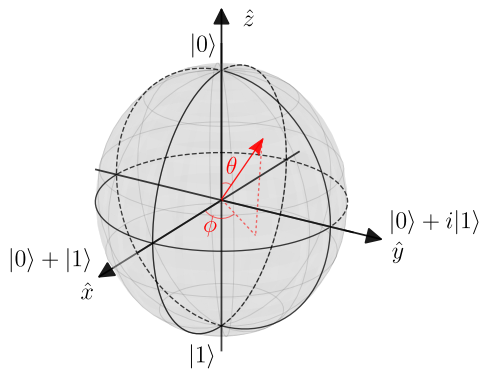
\includegraphics[width=0.35\textwidth]{figures/png/BlochSphere.png}
\caption{Example of qubit state representation on the Bloch sphere\\
Source: Metrology of Quantum Control and Measurement in Superconducting Qubits \cite{Chen2018}}
\label{fig:BlochSphere}
\end{figure}

The qubit states $\ket{0}$ and $\ket{1}$ can also be associated with energy eigenstates of a physical system, where $\ket{0}$ represents the ground state with energy $E_0$ and $\ket{1}$ represents the excited state with energy $E_1$, assuming $E_0 < E_1$. 
In this energy eigenbasis, the Hamiltonian of the qubit is given by
\begin{equation}\label{eq:qubithamiltonian}
    \hat{H}_q = E_0 \ket{0} \bra{0} + E_1 \ket{1} \bra{1} = 
    \begin{pmatrix}
        E_0 & 0 \\
        0 & E_1
    \end{pmatrix}.
\end{equation}

Since only energy differences are physically relevant, it is possible to redefine the zero-point energy by subtracting the constant term $E_0 (\ket{0} \bra{0} + \ket{1} \bra{1})$, leading to the simplified Hamiltonian
\begin{equation}\label{eq:qubithamiltonian}
    \hat{H}_q = (E_1 - E_0) \ket{1} \bra{1} = \hbar \omega_q \ket{1} \bra{1} = \hbar \omega_q \hat{\sigma}^{+} \hat{\sigma}^{-} = 
    \begin{pmatrix}
        0 & 0 \\
        0 & \hbar \omega_q
    \end{pmatrix},
\end{equation}

where $\omega_q = (E_1 - E_0)/\hbar$ is the qubit transition frequency, and we have used the relation $\hat{\sigma}^{+} \hat{\sigma}^{-} = \ket{1} \bra{1}$.
For convenience, the Hamiltonian can also be rewritten in terms of the Pauli $z$-matrix, $\hat{\sigma}_z$, by adding a term proportional to the identity:
\begin{equation}
    \hat{H}_q = \hbar \omega_q \ket{1} \bra{1} - \frac{\hbar \omega_q}{2}\mathbb{I} = 
    \begin{pmatrix}
        -\frac{\hbar \omega_q}{2} & 0 \\
        0 & \frac{\hbar \omega_q}{2}
    \end{pmatrix} = -\frac{\hbar \omega_q}{2} \hat{\sigma}_z.
\end{equation}

\paragraph{}
Qubits can be implemented through various physical mechanisms; however, their practical realization remains a significant challenge due to their susceptibility to environmental interactions, which lead to decoherence and reduce their coherence time. 
Despite the diversity of possible physical implementations, any functional quantum computing system must satisfy a set of fundamental criteria. 
These requirements, known as the DiVincenzo criteria, establish the essential conditions for the construction and operation of a viable quantum computer \cite{DiVincenzo_2000}, \cite{manenti_quantum_2023}:
\begin{enumerate}
    \item The physical system used as quantum computer must comprise a set of qubits, meaning that the quantum system must be well-characterized, and scalable such that quantum
    computing can be realized.
    \item It must be possible to initialize the qubits in a reliable state, such as the ground state.
    \item The coherence time of the qubits must be longer than the typical gate time, ideally should be possible to perform $>10^4$ operations, that is the number which allows for realizing effective error corrections.
    \item It must be possible to implement a universal set of quantum gates.
    \item It must be possible to measure the qubits in the computational basis.
\end{enumerate}

In the present work, I will focus on superconducting qubits, which constitute the hardware I have worked on and where the experiments were conducted. 
However, several of the experiments described later can also be implemented using different physical systems.

\section{Transmon qubits}
In this section, I provide a review of the structure and operation of superconducting transmon qubits. 
The content of this section is based on the \textit{Quantum Information Science} manual \cite{manenti_quantum_2023}, \textit{The Metrology of Quantum Control and Measurement in Superconducting Qubits} \cite{Chen2018}, the notes from quantum computing lectures held by Professor Olivares \cite{Olivares2021}, and the original transmon paper \cite{TransmonPaper}.

\subsection{Josephson Junctions}
The Josephson junction (JJ) is formed by a thin oxide layer positioned between the two superconductors which acts as an insulating barriers. 
An example of Josephson junction is show in figure \ref{fig:JJ}, a side view in image \ref{fig:JJ_side} and a top view in image \ref{fig:JJ_top}.
\begin{figure}[ht!]
    \centering
    \begin{subfigure}{0.45\textwidth}
        \centering
        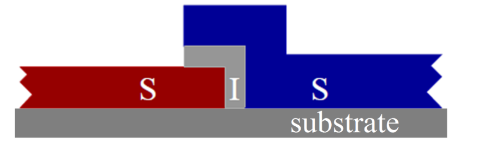
\includegraphics[width=0.90\textwidth]{figures/png/JJ_side.png}
        \subcaption{}
        \label{fig:JJ_side}
    \end{subfigure}
    \hfill
    \begin{subfigure}{0.45\textwidth}
        \centering
        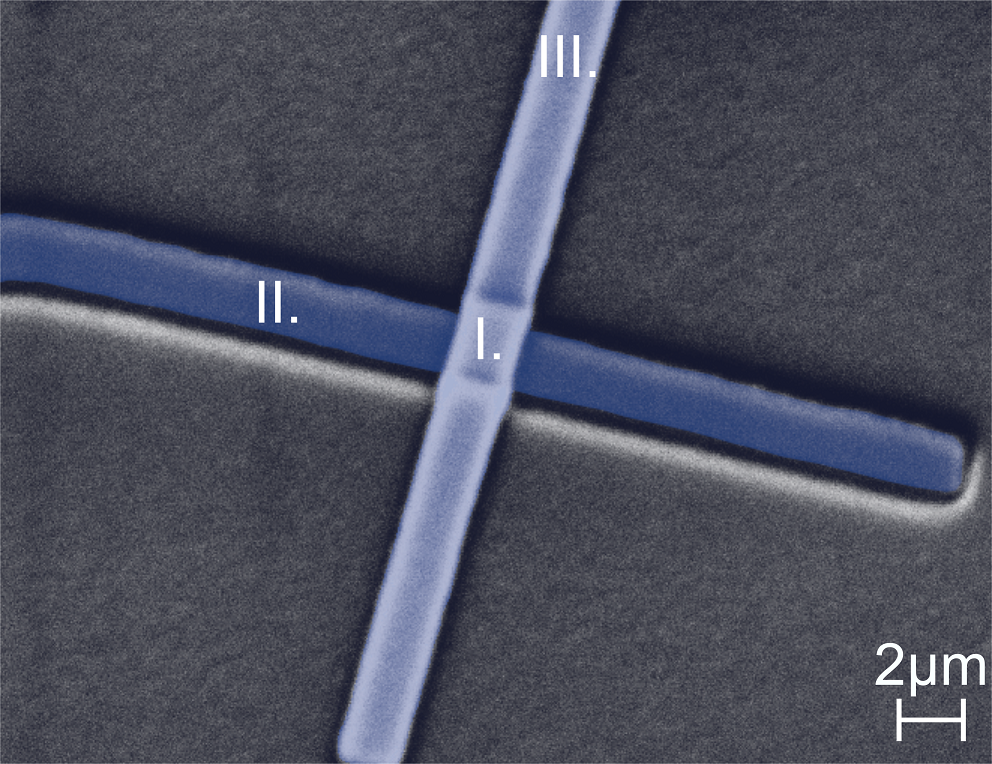
\includegraphics[width=0.70\textwidth]{figures/png/JJ_top.png}
        \subcaption{}
        \label{fig:JJ_top}
    \end{subfigure}
    \caption{Figure \ref{fig:JJ_side}: Side viwe of a Josephson junction, the two superconducting pads are coloured in red and blue and indicating by the letter S. In grey, indicated by letter I is represented the insulating barrier of oxide. 
    The superconductors and the oxide are layered over a substrate.\\
    Figure \ref{fig:JJ_top}: Electron microscope image of a $2 \mu\text{m} \cross 2 \mu\text{m}$ cross-type junction: I. Josephson junction. II. Base electrode. III. Contact to the top electrode.\\
    Source:\url{https://www.ims.kit.edu/english/2551.php}}
    \label{fig:JJ}
\end{figure}

Superconductivity is a phenomenon observed in certain materials where, when cooled well below a critical temperature $T_c$, which depends on the material, their electrical resistance drops to zero, allowing them to behave as perfect conductors.
According to the BCS (Bardeen-Cooper-Schrieffer) theory, superconductivity arises, from the formation of Cooper pairs, which are bound states of electrons with opposite momenta and spins.
These pairs collectively forms a macroscopic quantum states described by a single waveform $\psi(\mathbf{r})$ which can be expressed as 
\begin{equation}\label{eq:BCSequation}
    \psi(\mathbf{r}) = \sqrt{\rho(\mathbf{r})}e^{i\theta(\mathbf{r})}
\end{equation}
where $\rho(\mathbf{r})$ is the density of Cooper pairs in the metal, which is typically uniform in the bulk of the superconductor, and $\theta(\mathbf{r})$ is the macroscopic phase of the superconducting wavfunction.

For this reason the wavefunctions on the two sides of the JJ can be denoted as
\begin{equation}\label{eq:JosephsonWavefunctions}
    \psi_1(\mathbf{r}, t) = \sqrt{\rho_1(\mathbf{r}, t)} e^{i\theta_1(\mathbf{r},t)}, \psi_2(\mathbf{r}, t) = \sqrt{\rho_2(\mathbf{r}, t)} e^{i\theta_2(\mathbf{r},t)}
\end{equation}

The dynamics of the system can be described by the two equations\begin{equation}\label{eq:schr1}
    i\hbar \frac{d\psi_1}{dt} = E_1 \psi_1 + K \psi_2,
\end{equation}
\begin{equation}\label{eq:schr2}
    i\hbar \frac{d\psi_2}{dt} = E_2 \psi_2 + K \psi_1.
\end{equation}
By substituting the expression of $\psi_i$ into the Schr\"odinger equation \ref{eq:schr1}, \ref{eq:schr2} we obtain
\begin{equation}\label{eq:schr-sub1}
    \frac{d\rho_1}{dt} = \frac{2K}{\hbar} \sqrt{\rho_1 \rho_2} \sin(\theta_2 - \theta_1),
\end{equation}
\begin{equation}\label{eq:schr-sub2}
    \frac{d\rho_2}{dt} = -\frac{2K}{\hbar} \sqrt{\rho_1 \rho_2} \sin(\theta_2 - \theta_1).
\end{equation}

Since the derivative of the charge density is the current, from equations \ref{eq:schr-sub1} and \ref{eq:schr-sub2} we obtain the first Josephson equation
\begin{equation}\label{eq:Josephson1}
    I=I_c\sin{\phi}
\end{equation} 
where $I_c = \frac{2K}{\hbar}\sqrt{\rho_1\rho_2}$ is the critical current and $\phi$ is the superconducting phase difference $\theta_2 - \theta_1$.

Instead, from the real part of the Schr\"odinger equation \ref{eq:schr1}, \ref{eq:schr2} and a few calculations, we obtain the second Josephson equation
\begin{equation}\label{eq:Josephson2}
    \frac{d\phi}{dt} = \frac{2e}{\hbar} V(t).
\end{equation}
which can be rewritten as \begin{equation}
    \frac{d\phi}{dt} = \frac{2\pi}{\Phi_0} V(t).
\end{equation}
where $\Phi_0 = \frac{h}{2e}$ is the superconducting flux quantum, with $h$ is the Planck's constant and $2e$ is the charge of a Cooper pair.

The time derivative of the first Josephson equation \ref{eq:Josephson1} yields:
\begin{equation}\label{eq:current_derivative}
    \dot{I_J}=I_C\cos{\phi}\frac{\partial \phi}{\partial t},
\end{equation}
equation \ref{eq:current_derivative} suggests a nonlinear relation between the current the voltage. 
Using the Josephson voltage-phase relation and the fact that $\dot{I}=\frac{V}{L}$ it is possible to define an effective nonlinear inductance for the Josephson junction:
\begin{equation}\label{eq:LJ}
    L_J = \frac{1}{\cos{\phi}}\frac{\Phi_0}{2\pi I_c}.
\end{equation} 

In addition to ths inductive behaviour the Josephson junction also exibits capacitive properties due to its inherent capacitance $C_J$ with a corresponing energy of 
\begin{equation}\label{eq:capacitive_energy}
    E_{C_J} = \frac{Q^2}{2C_J}
\end{equation}.

Fom equation \ref{eq:LJ} it is possible to compute the energy stored in the nonlinear inductance as
\begin{align}\label{eq:inductive_energy}
    E_{L_J} &= \int_{0}^{t}\text{d}\tau I_J(\tau)V(\tau) = \int_{0}^{t}\text{d}\tau I_c\sin{\phi(\tau)}\frac{\partial\phi(\tau)}{\partial\tau}\frac{\Phi_0}{2\pi}\\
    &= \frac{\Phi_0 I_c}{2\pi}(1-\cos{\phi}) = E_J(1-\cos{\phi})
\end{align}
where $E_J$ represents the energy due to the behaviour of the junction as nonlinear inductor .

\subsection{CPB qubit}

A first example of superconducting qubit is the Cooper Pair Box (CPB), which consists of a small superconducting island connected to a reservoir of superconducting electrons through a Josephson junction \cite{Vion2002}, with an external gate voltage controlling the charge state.
The circuit corresponding to CPB is similar to the circuit of a parallel resonator where the linear inductance is subsituted by a Josephson junction which simply acts as a nonlinear inductance.

Combining the energy associated to the capacitance $C$ and the energy of the Josephson junction \ref{eq:inductive_energy} it is possible to write the classical Hamiltonian of the circuit
\begin{equation}\label{eq:CPB_hamiltonian}
    H_J = 4E_C n^2 - E_J\cos{\phi}
\end{equation}
where the constant term was ignored as it acts simply as a constant offset without influencing the dynamics of the system and where $E_C$ is the charging energy defined as \begin{equation}\label{eq:charging_energy}
    E_C = \frac{e^2}{2C}.
\end{equation}

\begin{figure}[ht!]
    \centering
    \begin{subfigure}{0.45\textwidth}
        \centering
        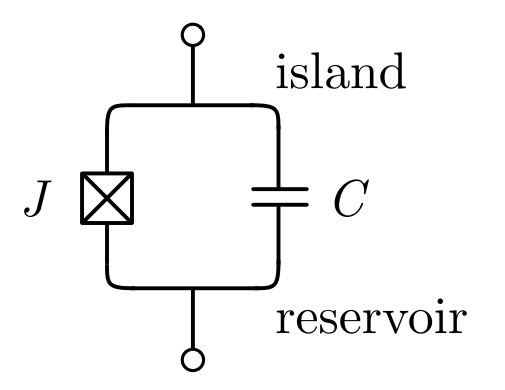
\includegraphics[width=0.60\textwidth]{figures/png/CPB.png}
        \subcaption{}
        \label{fig:CPB}
    \end{subfigure}
    \hfill
    \begin{subfigure}{0.45\textwidth}
        \centering
        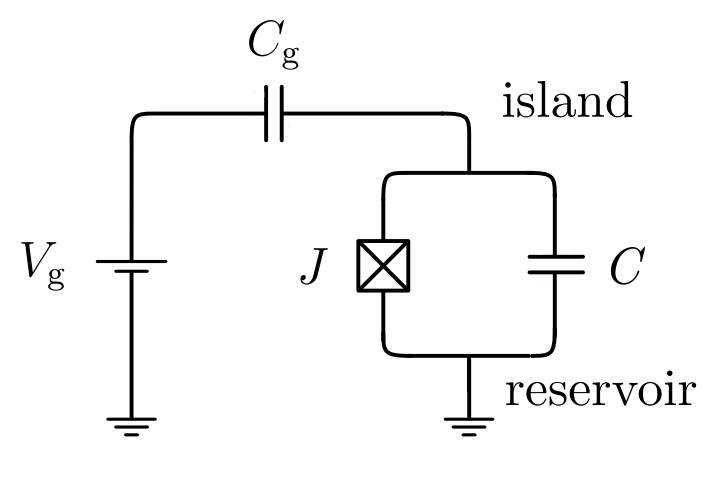
\includegraphics[width=0.70\textwidth]{figures/png/CPB_circuit.png}
        \subcaption{}
        \label{fig:CPB_circuit}
    \end{subfigure}
    \caption{Figure \ref{fig:CPB}: corresponding circuit of a CPB which consists of Josephson junction shunted by a capacitor. Surce: \cite{manenti_quantum_2023}. Figure \ref{fig:CPB_circuit}: electrical circuit of a CPB capacitively coupled to a DC voltage source through a capacitor $C_g$. Source: \cite{manenti_quantum_2023}.}
    \label{fig:CPB_general}
\end{figure}

To control the number of Cooper pairs on the island, it is possible to connecnt a DC voltage source $V_g$ to the system through a gate capacitor $C_g$, as shown in Figure \ref{fig:CPB_circuit}.
When $V_g = 0$, both the gate and qubit capacitors remain uncharged. 
As $V_g$ increases, a charge $Q_g = C_g V_g$ accumulates on the gate capacitor, inducing an equal and opposite charge on the island to maintain charge neutrality. 
When $Q_g \approx 2e$, a Cooper pair tunnels from the reservoir to the island, discharging the qubit capacitor. \\

The presence of the external voltage source introduces an additional control parameter for the number of Cooper pairs on the island, modifying the system's Hamiltonian. 
The resulting Hamiltonian of the Cooper Pair Box (CPB) takes the form

\begin{equation}\label{eq:CPB_complete}
    \hat{H} = 4E_C(\hat{n} - n_g)^2 - E_J \cos{\hat{\phi}}
\end{equation}

where $n_g = \frac{C_g V_g}{2e}$ represents the normalized gate charge.

A key feature of the system is the presence of a Josephson junction in place of a linear inductance. 
Unlike a standard LC circuit—corresponding to a quantum harmonic oscillator—this results in a non-equidistant energy level spectrum. 
In particular, the energy levels are anharmonic, allowing the first two levels to be spectrally isolated from the higher ones. 
This anharmonicity enables the use of the subspace spanned by the ground state $\ket{0}$ and the first excited state $\ket{1}$ aas a qubit.

The qubit frequency is defined as the frequency associated with the energy difference between these two states: $f_{01}(n_g) = f_Q = \frac{(E_1 - E_0)}{h}$.
This frequency can be tuned by varying the externally applied DC voltage, which modifies the system’s parameters and, consequently, its energy level spacing.\\

%%%NOTA PER ME: INSERIRE IL PLOT DEI LIVELLI ENERGETICI DEL CPB


\subsection{Transmon qubit}
One of the main drawbacks of the Cooper Pair Box (CPB) qubit, which ultimately led to its replacement by other qubit architectures, is its limited coherence time. 
The transmon qubit was introduced specifically to address this issue, with the goal of improving the dephasing time of the CPB. The key idea behind the transmon is to reduce the sensitivity of the energy levels to fluctuations in the gate charge—effectively flattening the energy bands—by increasing the ratio between the Josephson energy $E_J/E_C \geqq 1$,
this architecture was first proposed in \cite{TransmonPaper}, the first and more straightforward method to increase this ratio is to enlarge the capacitance of the qubit, which reduces the charging energy $E_C$.

Since the CPB and the transmon qubit have the same electrical circuit they are also described by the same hamiltonian \ref{eq:CPB_hamiltonian}. 
The difference is that in this case the transmon satisfies the condition $E_J/E_C \geqq 1$ it is possible to expand the cosine term in \ref{eq:CPB_hamiltonian} with a Taylor series and neglect the higher order terms:
\begin{equation}\label{eq:approx_transmon}
    \hat{H}\approx 4E_C\hat{n}^2 + \frac{1}{2}E_J\hat{\phi}^2 - \frac{E_J}{4!}\hat{\phi}^4
\end{equation}
where the last term, proportional to $\hat{phi}^4$, makes the potential of the transmon slightly anharmonic.

As happens in the standard harmonic oscillator case, the operators $\hat{phi}$ and $\hat{n}$ satisfy the cnaonical commutation relation $[\hat{\phi},\hat{n}]=i\mathbb{I}$, it is possible to introduce the raising and lowering operators $\hat{b},\hat{b}^\dagger$ as
\begin{equation}\label{eq:raising_lowering_operators}
    \hat{\phi} = \sqrt{\xi}(\hat{b}+\hat{b}^\dagger), 2\quad \hat{n} = -\frac{i}{2\sqrt{xi}}(\hat{b}-\hat{b}^\dagger),
\end{equation}
where $\xi =  \sqrt{2E_C/E_J}$.

Substituting equations \ref{eq:raising_lowering_operators} in the hamiltonian, equation \ref{eq:approx_transmon} becomes
\begin{equation}\label{eq:transmon_hamiltonian}
    \hat{H} = \sqrt{8E_JE_C}\hat{b}^\dagger\hat{b} - \frac{E_C}{12}(\hat{b}+\hat{b}^\dagger)^4.
\end{equation}

Given equation \ref{eq:transmon_hamiltonian} it is possible to solve the eigenvalue proble $\hat{H}\ket{k}=E_k\ket{k}$ and calculate the energy levels $E_k$.
The first term of hamiltonian \ref{eq:transmon_hamiltonian} is the harmonic oscillator contribution with eigenstates $\ket{k}$ and eigenvalues $\sqrt{8E_JE_C}k$. 
Since $E_C \ll E_J$, the second term $ \hat{V} = -\frac{E_C}{12}(\hat{b} + \hat{b}^\dagger)^4$ represents a small perturbative contribution to the Hamiltonian and can be treated using perturbation theory. 
The first-order correction to the energy levels is given by the diagonal matrix elements of the perturbation operator: $\Delta E_k^{(1)} = \langle k | \hat{V} | k \rangle$.
It is possible to verify that $\bra{k} \hat{V} \ket{k} = -\frac{E_C}{12} (6k^2 + 6k + 3)$. 
Thus the eigenenergies of the transmon hamiltonian are 
\begin{equation}
    E_k \approx \sqrt{8E_JE_C}k - \frac{E_C}{2}(k^2 + k).
\end{equation}

As mentioned before, the qubit frequency is defined as $f_Q = f_{01} = (E_1 - E_0)/h$ which yields
\begin{equation}
    f_01 \approx (\sqrt{8E_JE_C} - E_C)/h
\end{equation}

As explained at the beginning of this section, a large $E_J/E_C$ ratio makes the transmon qubit significantly less sensitive to charge noise. 
However, this improvement comes at the expense of reduced anharmonicity in the energy level spectrum. 
The anharmonicity $\eta$ is defined as the difference between the second and first transition energies, relative to the first transition energy:
\begin{equation}
    \eta = \frac{(E_2 - E_1) - (E_1 - E_0)}{\hbar} = \omega_{12} - \omega_{01}.
\end{equation}
For a transmon, the anharmonicity $\eta$ is negative, reflecting the fact that the level spacing decreases with increasing energy. 
Ideally, the absolute value  $|\eta|$ should be sufficiently large to allow external microwave drives to selectively address the $\ket{0}\leftrightarrow\ket{1}$ transition without inadvertently exciting higher-energy states.


\subsection{Flux-tunable transmon}
To implement certain two-qubit gate schemes, such as swap interactions, it is essential to tune the qubit frequency. 
A common approach to achieving this is by adding an extra junction to the transmon, the most common configuration is the SQUID (Superconducting QUantum Interference Device).
In the SQUID configuration two Josephson junctions are connected in parallel on a superconducting loop as shown in Figure [??].

Starting from the Hamiltonian of the single Josephson junction it is possible to write the hamiltonian of a SQUID:
\begin{equation}\label{eq:SQUID_Hamiltonian}
    \hat{H} = 4E_C\hat{n}^2 - E_{J1}\cos{\hat{\phi_1}} - E_{J2}\cos{\hat{\phi_2}}
\end{equation}
where $E_{J1}$ and $E_{J2}$ are the Josephson energies of the two junctions, and the operators $\hat{\phi_1}$ and $\hat{\phi_2}$ are the phase differences across the junctions.

Because od the quantization of the magnetic flux through the SQUID, the quantities $\hat{\phi_1}$ and $\hat{\phi_2}$ are not independet. 
In particular, as show in \cite{manenti_quantum_2023}, the difference between $\hat{\phi_1}$ and $\hat{\phi_2}$ follows the following relation:
\begin{equation}\label{eq:phases_relation}
    \hat{\phi_1} - \hat{\phi_2} = \frac{2\pi}{\Phi_0}\Phi_{\text{ext}}\mathbb{I}(\text{mod}2\pi)
\end{equation}
where $\Phi_{\text{ext}}$ is the flux of external magnetic field defined as the integral of the magnetic field over the SQUID area.

Equation \ref{eq:phases_relation} can be simplified and rewritten as 
\begin{equation}\label{eq:tunable_transmon_hamiltonian}
    \hat{H} = 4E_C\hat{n}^2 - E_J(\Phi_{\text{ext}})\cos{\hat{\varphi}}
\end{equation}
where $\hat{\varphi} = \frac{\hat{\phi_1}+\hat{\phi_2}}{2}$, and the Josephson energy is flux-dependent: 
\begin{equation}\label{eq:EJ_tunable}
    E_J(\Phi_{\text{ext}}) = (E_{J1} + E_{J2}) \left| \cos \left( \pi \frac{\Phi_{\text{ext}}}{\Phi_0} \right) \right| \sqrt{1 + d^2 \tan^2 \left( \pi \frac{\Phi_{\text{ext}}}{\Phi_0} \right) },
\end{equation}
where $d = \frac{E_{J1}-E_{J2}}{E_{J1}+E_{J2}}$ is the relative junction asymmetry.

Then, it's easy to see that the frequency $f_Q$ of a two-junction transmon dependends on the magnetic flux $\Phi_Q(t)$ through the SQUID loop, for symmetric junctions is given by
\begin{equation}\label{eq:freqdepndenceonflux}
    f_Q(\Phi_Q) \approx \frac{1}{h} \left( \sqrt{8E_J E_C \cos\left(\pi \frac{\Phi_Q}{\Phi_0} \right)} - E_C \right).    
\end{equation}

\begin{figure}[ht!]
    \centering
    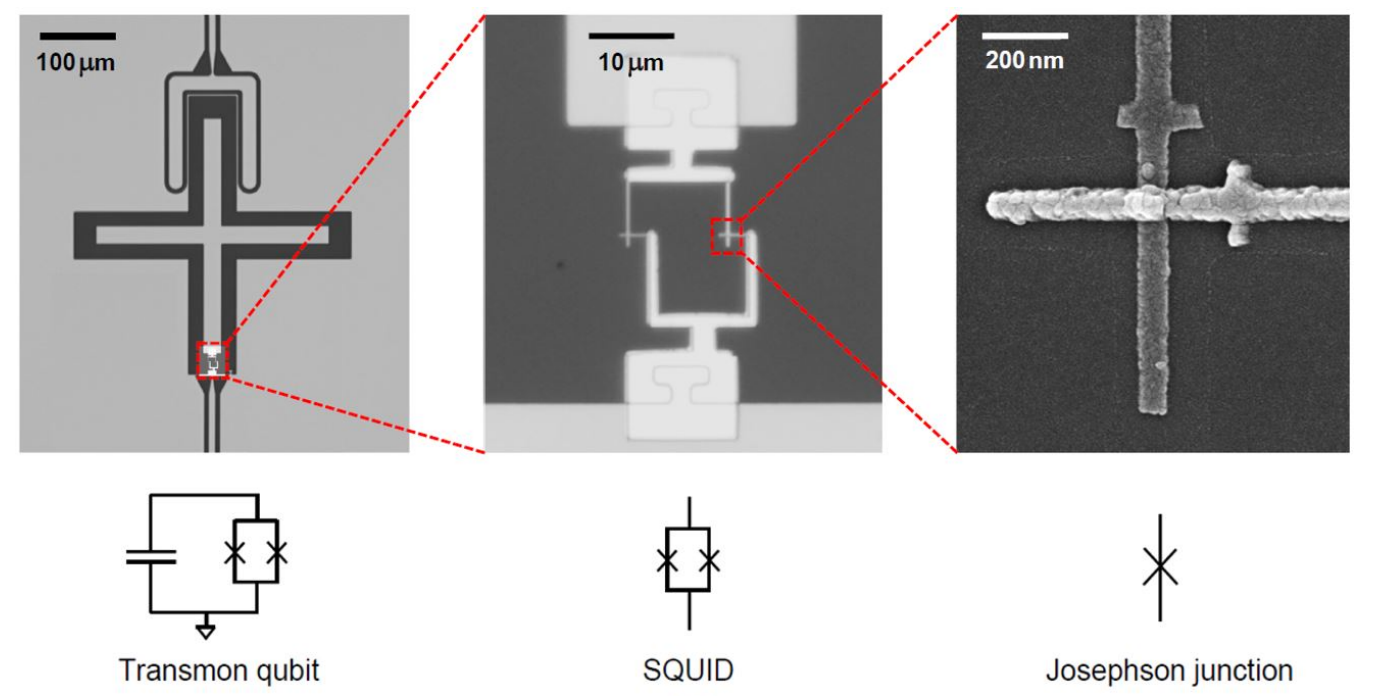
\includegraphics[width=0.50\textwidth]{figures/png/FrequencyTunableTransmon.png}
    \caption{Images of a flux tunable transmon qubit. From left to right: the flux tunable transmon qubit, consisting of a large cross-shaped capacitance in parallel with a SQUID to ground, and its corresponding circuit. A zoom in of the SQUID (center), a single Josephson junction (right). Source: \cite{Roth_2023}}
    \label{fig:FrequencyTunableTransmon}
\end{figure}


\section{Circuit QED}\label{sec:cQED}
Up to this point, I have discussed the physical structure of a transmon qubit. 
However, in order to perform quantum computing, it is essential to be able to control and measure its quantum state.
One approach to achieve this is to capacitively couple the qubit to both a drive line and a readout line. 
The drive line is used to manipulate the state of the qubit, while the readout line is employed to measure it.
An example of such a system is shown in Figure \ref{fig:Transmon_model}, along with the corresponding circuit diagram.

\begin{figure}[ht!]
    \centering
    \begin{subfigure}{0.47\textwidth}
        \centering
        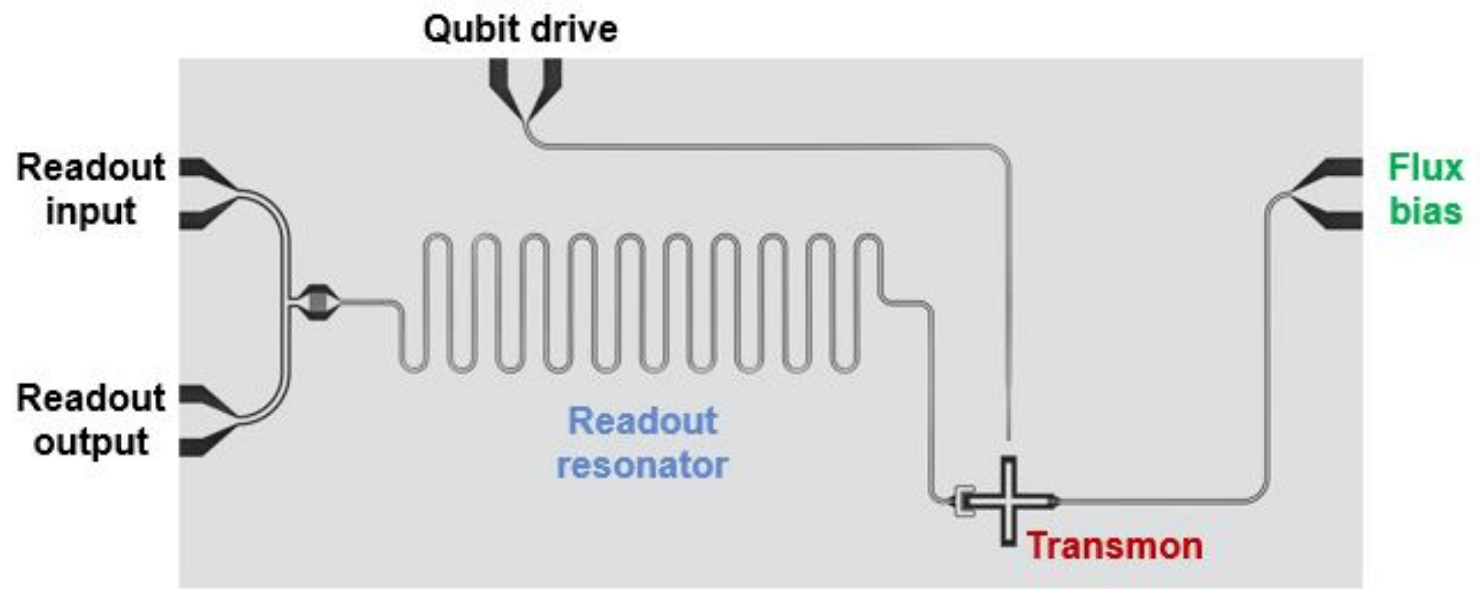
\includegraphics[width=\textwidth]{figures/png/TransmonBoard.png}
        \subcaption{}
        \label{fig:TransmonBoard}
    \end{subfigure}
    \hfill
    \begin{subfigure}{0.47\textwidth}
        \centering
        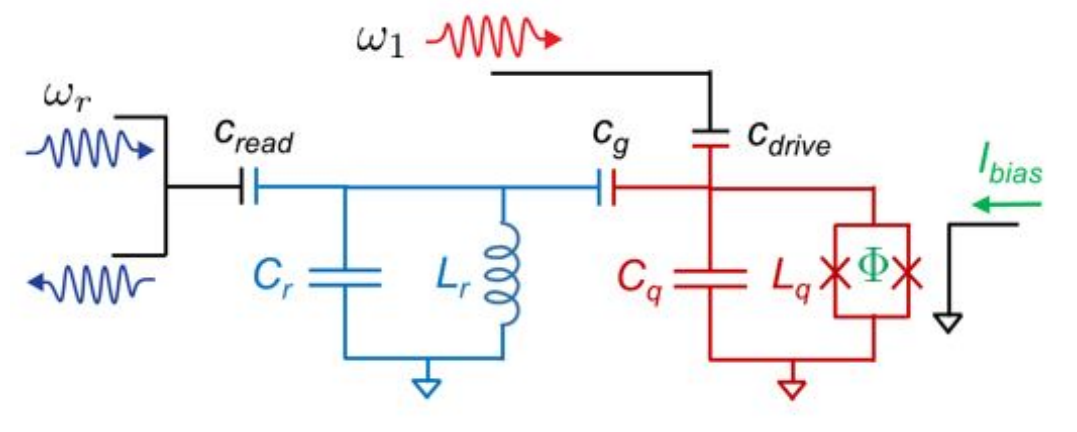
\includegraphics[width=\textwidth]{figures/png/TransmonCircuit.png}
        \subcaption{}
        \label{fig:TransmonCircuit}
    \end{subfigure}
    \caption{Figure \ref{fig:TransmonBoard} shows an example of a single transmon device. Figure \ref{TransmonCircuit} shows the equivalent lumped element circuit model of the device in \ref{fig:TransmonBoard}. Source: \cite{Roth_2023}}
    \label{fig:Transmon_model}
\end{figure}

\subsection{Qubit readout}

%In the architecture of circuit quantum electrodynamics (cQED), these requirements are addressed by exploiting the dispersive interaction between the qubit and a far-detuned microwave resonator

\subsection{Qubit control}
%Posso rappresentatre l'operatore densità come una matrce 2x2, mi serve per dopo, per la descrizione del depolarizing channel
A quantum operation is a mathematical transformation that describes how a quantum state changes as a consequence of a physical process. Formally, it is a map $\mathcal{E}$ that transforms a quantum state described by a density operator $\hat{\rho}$ into another state described by a new density operator $\hat{\rho}'$:
\begin{equation}
    \mathcal{E}(\rho) = \rho'\label{eq:quantum_map}.
\end{equation}

The simplest example of a quantum operation is the evolution of a quantum state $\hat{\rho}$ of a closed quantum system, under a unitary operator $\hat{U}$, which can be written as $\mathcal{E} \equiv \hat{U} \hat{\rho} \hat{U}^{\dagger}$.

\paragraph{Depolarizing channel}
A depolarizing channel describes a process in which the current state of the $n$-qubit system $\rho$, is replaced by $\frac{\id}{2^n}$, with probability $d$. This process can be represented with a quantum map as follows:
\begin{equation}
    \mathcal{E}_{dc}(\rho) = d\frac{\id}{2^n}+(1-d)\rho\label{eq:depolarizing_channel}
\end{equation} 


\subsection{Rabi experiments}


